\section{Experiments run after the held-out tests}
\label{app:followup}
We ran these experiments after both held-out tests. None changes a conclusion of the main text.

\subsection{Compiled edit versus an activation hook}
\label{app:hook}
We compare three ways to apply the same edit at the same held-out first-edit decisions. (A) is the compiled adapter as served. (N) is a hook that adds the intended neuron write $\gelu(g \cdot \hat{x})\,(u \cdot \hat{x})\, v$ to the MLP output of the three layers, with $\hat{x}$ the normalised MLP input. (V) is a hook that adds the constant or gate-scaled vector $m\, d_l$ to the layer output, as in activation addition. For the one edited neuron per layer, the adapter stores the edited gate row, up row and down column minus the dequantised 4-bit base weights. It is applied unmerged on top of the 4-bit weights. We run the control the same three ways. For explore-more, this is the matched random control. For the gate, it is Claude's ungated 0.125-gap random control, whose predicted shift is about one-fifth of the gate's. Part~1 teacher-forces the logged completion through a reimplementation of the deployed forward pass (4-bit weights, bfloat16) on 76 decision points. It compares residual changes at all positions and next-token distributions. Part~2 regenerates the decision greedily with the dense checkpoint in a second framework, on 57 points, for always-on explore-more.

\begin{table}[h]
\caption{Compiled adapter (A) against a neuron-write hook (N) and a vector-addition hook (V); mean over 76 held-out decision points. Cosines and $R^2$ compare the change from the unedited model in the residual stream at the stated layer; intervals on the cosines are within $\pm 0.003$.}
\label{tab:hook}
\centering
\small
\resizebox{\linewidth}{!}{\begin{tabular}{lrr}
\toprule
 & Explore-more 0.25 & Before-first-edit gate \\
\midrule
Cosine A vs N, layers 18 / 22 / 41 \up & 0.992 / 0.992 / 0.972 & 0.994 / 0.996 / 0.984 \\
Norm ratio A / N, layer 41 & 1.001 & 1.000 \\
$R^2$ A vs N, layers 18 / 41 \up & 0.984 / 0.945 & 0.989 / 0.968 \\
Cosine A vs V, layers 18 / 22 / 41 & 0.949 / 0.804 / 0.946 & 0.955 / 0.731 / 0.945 \\
Cosine A vs control, layer 41 & 0.056 & 0.018 \\
Projection on write direction$^{b}$ / class gap, layer 18: A / N / V & 0.236 / 0.236 / 0.250 & 0.249 / 0.249 / 0.265 \\
KL(unedited $\Vert$ A), completion tokens & 0.0112 & 0.0127 \\
KL(unedited $\Vert$ A), decision position & $3.4\times10^{-5}$ & $3.4\times10^{-5}$ \\
KL(N $\Vert$ A) \dn & 0.00011 & 0.00012 \\
KL(V $\Vert$ A) \dn & 0.00039 & 0.00051 \\
KL(unedited $\Vert$ control)$^{a}$ & 0.0029 & 0.0056 \\
\bottomrule
\end{tabular}}

\smallskip
\raggedright\footnotesize $^{a}$ Gate column: Claude's ungated 0.125-gap control. It writes at every position, unlike the gate, so it is not gate-matched. KL rows are over the positions that predict completion tokens (about 870 per point) unless marked ``decision position''. $^{b}$ The unit direction that the edit writes along at that layer, not the signed class direction $d$, so a positive value is a shift in the intended sense.
\end{table}

The compiled adapter reproduces the hooked neuron write. Its next-token distribution is about 100 times closer to the hook's than to the unedited model's (Table~\ref{tab:hook}). A plain vector addition is a looser match, most visibly at layer 22 (cosine 0.80 and 0.73). At the decision position itself, the gate's adapter--hook cosine at layer 18 is 0.883 (one point at 0.044). The output distributions there still agree closely (gate: KL(N$\,\Vert\,$A) $7.9\times10^{-7}$ against KL(unedited$\,\Vert\,$A) $3.4\times10^{-5}$). At the decision position, the edits' own KL ($3.4\times10^{-5}$ for both) is about 330 to 370 times smaller than over the completion tokens (0.0112 and 0.0127). Regeneration covered 57 points for always-on explore-more only, too few to detect the edit's own effect, and it does not separate the adapter from either hook. Over these 57 points, the share of decisions that are edits is 0.632 unedited, 0.614 for A, 0.544 for N and 0.632 for V. The difference N minus A is $-0.070$ (95\% CI $-0.153$ to $+0.013$). N agrees with A on the tool chosen at 86\% of points, close to the unedited model's 88\%. On these 57 points the edit itself does not move the edit share (A minus unedited $-0.018$, CI $-0.109$ to $+0.074$), so this part does not rank the three. The two hooks differ from each other (N minus V $-0.088$, CI $-0.162$ to $-0.014$, uncorrected over 24 comparisons: 12 pairs, two metrics). The hooks reproduce the adapter's full output on 5 of 57 points, against 0 of 57 for the unedited model.

\textbf{Setup notes.} Part~1 covers 76 of the 320 planned points and runs in one framework. The 57 points of Part~2 are the 27 longest and 30 shortest prompts of the first 104. The hook adds in bfloat16. A replaces the overwritten neuron, while N adds a new neuron beside it. The remaining difference between A and N ($1 - R^2$ of 0.8 to 5.5\%, growing with depth) therefore combines the old neuron's output and numerical precision. Regeneration uses HF transformers with dense bfloat16 weights, which are identical to the dequantised 4-bit weights. In that framework the explore-more edit's decision-position KL between unedited model and adapter has mean 0.0065 over the 57 points (heavy-tailed), against $3.4\times10^{-5}$ in Part~1. For the gate's control, the vector hook (CV) matches the control adapter (C) poorly: the cosine between their residual changes is 0.12 at layer 18 and 0.42 at layer 20, and the adapter's change is about 7 and 2 times the hook's in norm. This control is ungated with a small intended shift (0.02 to 0.05 class gaps, against about 0.26 for the gate), so most of its adapter's change at these layers lies off the added vector. Its neuron hook still matches it (cosine 0.96 to 0.99). We ran regeneration for explore-more only.

\subsection{Round 2: dose, depth and gate variants of the before-first-edit gate}
\label{app:round2}
One author (Claude) built variants of its before-first-edit gate. We ran them in two batches, each with its own unedited arm. Table~\ref{tab:round2} lists every arm.

\begin{table}[h]
\caption{Round 2, 170 development tasks, one run per arm. ``Better / worse'' counts tasks solved by the arm and not by the unedited model of the same batch, and the reverse; $p$ is a two-sided sign test. Strength is in class gaps. One arm was stopped early.}
\label{tab:round2}
\centering
\small
\resizebox{\linewidth}{!}{\begin{tabular}{llrrrr}
\toprule
Batch & Arm & Solved \up & Unedited & Better / worse & $p$ \\
\midrule
29 & Before-first-edit gate, 0.25 (repeat) & 28 & 25 & 12 / 9 & 0.66 \\
29 & Same gate on five layers (16--24) & 28 & 25 & 13 / 10 & 0.68 \\
29 & Gate + layers 24--28 of Gemini's explore + concise edit & 28 & 25 & 10 / 7 & 0.63 \\
29 & Gate at strength 0.5 & 25 & 25 & 8 / 8 & 1.00 \\
29 & Gate at strength 1.0 (stopped at 96 tasks) & 2 of 96 & & & \\
\midrule
30 & Gate 0.25 + early-calls gate 0.3 & 33 & 28 & 13 / 8 & 0.38 \\
30 & Early-calls gate at strength 0.6 & 30 & 28 & 8 / 6 & 0.79 \\
30 & Early-calls gate (round-1 edit, repeat) & 28 & 28 & 9 / 9 & 1.00 \\
30 & Gate 0.5 + layers 24--28 of Gemini's edit & 21 & 28 & & \\
30 & Five-layer gate at strength 0.5 & 12 & 28 & & \\
\bottomrule
\end{tabular}}
\end{table}

A higher dose did not help. Strength 0.5 matched the unedited model on three layers and lost 16 tasks on five layers. Strength 1.0 solved 2 of its first 96 tasks. The best arm, the gate combined with the early-calls gate, was 5 tasks ahead in its one batch. This difference is within the spread of single batches.

\subsection{Round 3: stacking edits from different authors}
\label{app:round3}
We wrote predictions and a decision rule before any run. A stacked edit goes to a new held-out test only if it beats the unedited model by at least 8 tasks in the mean of two batches and by at least 5 in each, and beats a stacked control by at least 5.

\textbf{A plain sum of adapters is not a stack.} The authors' builders all overwrite the quietest neurons of a layer, so their edits share neurons. For example, every edit uses neuron 2972 of layer 20. A sum of two adapters therefore gives one neuron with mixed gate, up and down weights, not two neurons. With such sums, every stacked arm, the stacked control included, ended every episode without a submission. We stopped that batch after 3 to 18 tasks per arm and use none of its numbers. We rebuilt the stacks so that a later source's neuron moves to the next quietest free neuron of the layer and carries the source's exact edited weights.

\textbf{Result.} We stopped the two batches with the rebuilt stacks at 49 to 106 of 170 tasks per arm, so the decision rule is not evaluated. Table~\ref{tab:round3} gives the counts on the tasks completed by both an arm and the unedited model of its batch. Before this intersection, the unedited arm had completed 106 tasks in batch 33 and 82 in batch 34, and the other arms 56 to 106 and 49 to 84. The largest difference for a stack is $+3$ tasks over the two batches (gate plus Gemini's edit, 26 against 23). The stacked control is $+2$ (29 against 27). The other two stacks are behind (21 against 23, and 15 against 16). The repeat of the best round-2 arm is level with the unedited model (25 against 24 over the two batches).

\begin{table}[h]
\caption{Round 3: solved tasks among those completed by both the arm and the unedited model of the same batch (batches 33 and 34). The pre-registered rule needs complete batches and is not evaluated. The intersections (49 to 106 tasks) favour tasks that finish quickly and differ between arms.}
\label{tab:round3}
\centering
\small
\begin{tabular}{lrrrrrr}
\toprule
 & \multicolumn{3}{c}{Batch 33} & \multicolumn{3}{c}{Batch 34} \\
\cmidrule(lr){2-4}\cmidrule(lr){5-7}
Arm & Tasks & Arm & Unedited & Tasks & Arm & Unedited \\
\midrule
Gate + Gemini's explore-and-concise edit & 94 & 14 & 12 & 73 & 12 & 11 \\
Gate + early-calls gate + Gemini's edit & 83 & 12 & 12 & 73 & 9 & 11 \\
Same, writes scaled by 0.7 & 56 & 8 & 9 & 49 & 7 & 7 \\
Stacked control & 106 & 14 & 14 & 82 & 15 & 13 \\
Gate + early-calls gate (round-2 best, repeat) & 93 & 14 & 12 & 77 & 11 & 12 \\
\bottomrule
\end{tabular}
\end{table}

\subsection{Round 4: a wide screen motivated by the loss after long exploration}
\label{app:round4}
\textbf{Design, fixed before launch} (\texttt{round4\_predictions.md}, with six dated amendments). We wrote each amendment before the decision-rule batches were scored. Amendments 3 and 5 record partial scores of the batches they stop (b35 on 41 tasks, b46 on 57; 42 and 59 in the final logs, with the same conclusions). The diagnosis of \S\ref{sec:diagnosis} shows that episodes with 8 or more calls before the first file edit solve far less (odds ratio 0.12). The point estimates peak at 5--7 calls; that bin's interval includes 1. Earlier edits pushed only towards more exploration. Round 4 adds a ``commit late'' neuron that pushes towards the first edit once 8 or more calls have passed without one. We test it alone (\texttt{late30}, \texttt{late60}) and combined with the early explore push (\texttt{u*}, \texttt{pu}). We also test dose, depth and gate variants of the before-first-edit gate (\texttt{pe*}, \texttt{pre*}) and two random-direction family controls. This gives 20 adapters in four arm sets of five. Each batch has its own unedited arm, 170 development tasks and one rollout. Each edit has a written prediction: an interval of solved tasks relative to the unedited arm of its batch. Decision rule: an edit goes to a held-out test only if its mean gain over its two batches is at least 8 tasks, it gains at least 5 in each batch, and its mean gain exceeds its family control's by at least 5. We screen twenty edits, so any development $p$ value is Holm-corrected over 20. A secondary pooled analysis (per-edit paired difference summed over all its batches, task-level sign test, Holm over 20) is reported but cannot send an edit to a held-out test.

\textbf{Protocol notes.} Six of the first eight batches were relaunched within 20 minutes under new batch names to fit sandbox capacity. Batches that stopped before 170 tasks are scored on the tasks completed by every arm and marked incomplete. Batches ran at concurrency 4 per arm (35, 36, 45, 46), 6 (43, 44) or 8 (47--58). Every arm of a batch shares its setup, and we compare each edit only with the unedited arm of its own batch. Episodes have a 7.5-minute wall-clock limit, and we count session-limit rows per arm (Tables~\ref{tab:round4b} and~\ref{tab:round4}). Amendment~3 named batch 36 a decision-rule batch before it was scored, so we keep it at 156 tasks. That amendment replaced batch 35 with batch 45. Batch 46 was a third batch outside the rule. For the explore-plus-commit-late set (\texttt{u33}, \texttt{u36}, \texttt{u63}, \texttt{u33\_L5}, \texttt{u33\_c6}) and the depth and dose set (\texttt{pe\_L*}, \texttt{pre15}, \texttt{pre35}), the family control ran in a different batch. For these two sets, rule~3 compares across batches.

\textbf{Results.} No edit passes the pre-registered rule. In the first batch of each arm set (Table~\ref{tab:round4}), the best edits gained 5 tasks (two edits), and 6 in batch 36, against the rule's 8. No single-batch difference has $p < 0.17$ except one failure. The depth variant that writes at layer 14 solved 1 of 170 tasks in both batches (0 won and 22 lost in batch 44, 0 and 28 in batch 50): this edit breaks the model at that depth. The largest single-batch gain, $+7$, belongs to a random-direction control (\texttt{u33\_ctrl}, batch 36). The explore-gate family's control lost 4 in batch 43. Under the decision rule, each edit has two batches (first arm set: 45 and 47; second: 36 and 48; third: 43 and 49; fourth: 44 and 50; Table~\ref{tab:round4b} and Figure~\ref{fig:round4}). The best mean gains are $+5.0$ for \texttt{pe\_L5} ($+5$, $+5$), \texttt{pe\_lo} ($+4$, $+6$) and \texttt{u36} ($+1$, $+9$; the $+9$ has uncorrected $p = 0.049$), and $+4.5$ for \texttt{pe\_L20} ($+1$, $+8$). None reaches the required $+8$, so no edit passes and none goes to a held-out test. Most edited arms have more session-limit rows than the unedited arm of the same batch (for example \texttt{pe\_hi} 28 against 14 and \texttt{u33\_ctrl} 26 against 13 in Table~\ref{tab:round4b}). For 10 of the 20 adapters, the written interval (mean width 4.05 tasks) contains the measured two-batch mean. There are 5 misses above and 5 below; the largest is \texttt{pe\_L14}, $-25$ against 0 to $+3$. Two intervals stated relative to a three-layer version are resolved against its measured mean. Of the 40 single batches, 18 fall inside their intervals. The secondary pooled analysis (Amendment 4) sums each edit's paired differences over every batch it ran in, the replicate batches 51--58 included. It applies a task-level sign test with Holm correction over the 20 adapters. The largest pooled gain is \texttt{pe\_lo}: 39 tasks won and 17 lost over 678 task pairs ($+22$, $p = 0.005$, Holm-adjusted $p = 0.087$; \texttt{pe\_L14} has the smallest $p$, so the step-down multiplies \texttt{pe\_lo}'s $p$ by 19 of the 20). This gain does not survive correction. The next are \texttt{pe\_L20} $+15$ ($p = 0.086$), \texttt{pe\_L5} $+13$ ($p = 0.12$), \texttt{pe\_c6} $+10$ and the random-direction control \texttt{u33\_ctrl} $+10$. No adapter is significant after correction. The pooled analysis uses the replicate batches as of 4:27 PM ET (batch 58 at 103--110 tasks); it does not affect the decision-rule verdict. Round 6 (Appendix~\ref{app:round6}) is the pre-registered replication of \texttt{pe\_lo}.

\begin{table}[h]
\caption{Round 4, second batch of each arm set (batches 47--50, all complete): solved tasks against the unedited arm of the same batch; won / lost are discordant tasks; the last column counts rows that ended at the 7.5-minute session limit for the unedited arm / the edit.}
\label{tab:round4b}
\centering
\small
\begin{tabular}{llllrrrr}
\toprule
Batch & Tasks & Arm & Unedited & Arm & $\Delta$ & Won / lost & Limit rows \\
\midrule
47 & 170 & \texttt{u33} & 24 & 26 & +2 & 10 / 8 & 15 / 20 \\
47 & 170 & \texttt{u33\_L5} & 24 & 29 & +5 & 14 / 9 & 15 / 23 \\
47 & 170 & \texttt{u33\_c6} & 24 & 29 & +5 & 12 / 7 & 15 / 23 \\
47 & 170 & \texttt{u36} & 24 & 33 & +9 & 13 / 4 & 15 / 24 \\
47 & 170 & \texttt{u63} & 24 & 28 & +4 & 13 / 9 & 15 / 16 \\
\midrule
48 & 170 & \texttt{pre\_early} & 25 & 27 & +2 & 8 / 6 & 13 / 23 \\
48 & 170 & \texttt{late30} & 25 & 27 & +2 & 9 / 7 & 13 / 18 \\
48 & 170 & \texttt{late60} & 25 & 25 & 0 & 6 / 6 & 13 / 22 \\
48 & 170 & \texttt{pu} & 25 & 22 & $-3$ & 7 / 10 & 13 / 22 \\
48 & 170 & \texttt{u33\_ctrl} (control) & 25 & 26 & +1 & 9 / 8 & 13 / 26 \\
\midrule
49 & 170 & \texttt{pe\_L5} & 24 & 29 & +5 & 11 / 6 & 14 / 21 \\
49 & 170 & \texttt{pe\_c6} & 24 & 29 & +5 & 10 / 5 & 14 / 14 \\
49 & 170 & \texttt{pe\_ctrl} (control) & 24 & 24 & 0 & 6 / 6 & 14 / 20 \\
49 & 170 & \texttt{pe\_hi} & 24 & 27 & +3 & 9 / 6 & 14 / 28 \\
49 & 170 & \texttt{pe\_lo} & 24 & 30 & +6 & 10 / 4 & 14 / 13 \\
\midrule
50 & 170 & \texttt{pe\_L14} & 29 & 1 & $-28$ & 0 / 28 & 16 / 5 \\
50 & 170 & \texttt{pe\_L20} & 29 & 37 & +8 & 15 / 7 & 16 / 19 \\
50 & 170 & \texttt{pe\_L22} & 29 & 25 & $-4$ & 6 / 10 & 16 / 25 \\
50 & 170 & \texttt{pre15} & 29 & 27 & $-2$ & 6 / 8 & 16 / 15 \\
50 & 170 & \texttt{pre35} & 29 & 26 & $-3$ & 6 / 9 & 16 / 23 \\
\bottomrule
\end{tabular}
\end{table}

\begin{figure}[h]
\begin{center}
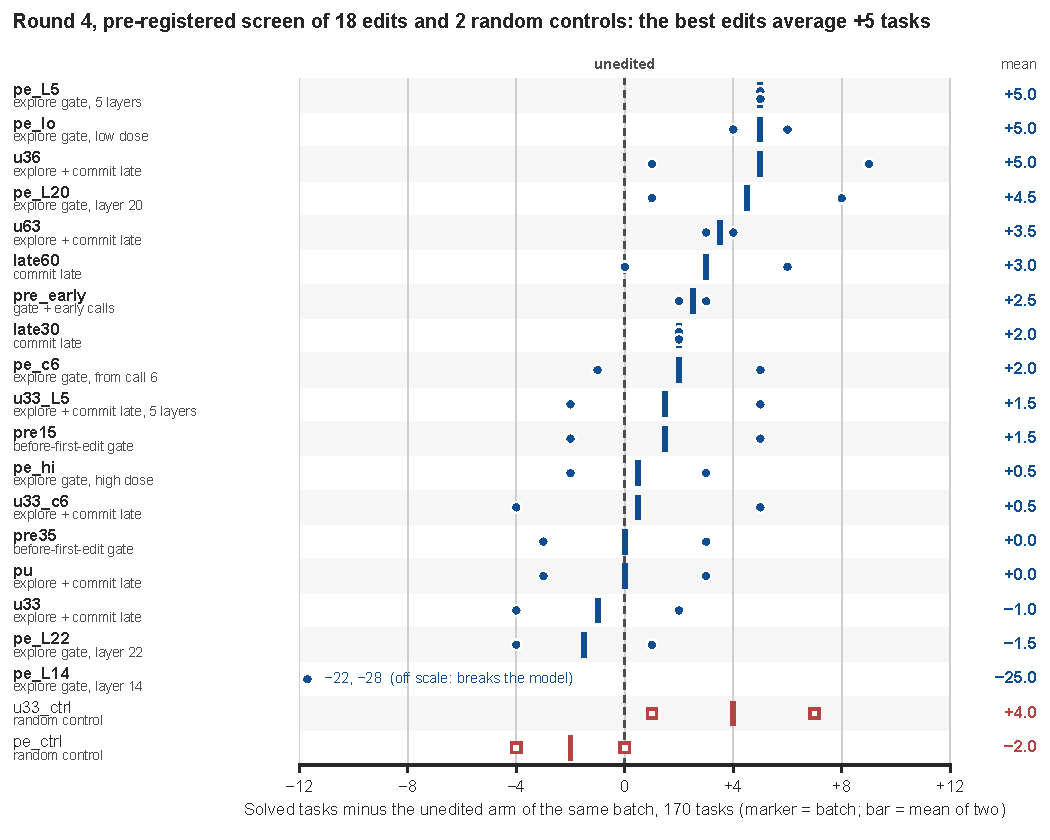
\includegraphics[width=1.0\linewidth]{figures/fig6_round4.pdf}
\end{center}
\caption{\textbf{Round 4: no edit reaches the pre-registered bar.} Each of the 18 edits and two random-direction controls in its two batches (first batch: 45, 36 [stopped at 156 tasks], 43 or 44; second: 47--50), as solved tasks minus the unedited arm of the same batch; bar = mean of the two. The pre-registered rule required a mean of at least $+8$, at least $+5$ in each batch and $+5$ over the family control. The layer-14 variant solved 1 of 170 in both batches (off scale).}
\label{fig:round4}
\end{figure}


\begin{table}[h]
\caption{Round 4, first batch of each arm set: solved tasks on the tasks completed by every arm of the batch, each arm against the unedited arm of its own batch; won / lost are discordant tasks, $p$ an exact two-sided sign test (shown when below 0.5). Batch 36 was stopped at 156 tasks complete in every arm (Amendment 6; arms had completed 158 to 166). Batches 35 (42 common tasks; arms 42 to 52) and 46 (59; arms 59 to 70) were stopped early and are not tabulated; intersections of stopped batches favour tasks that finish quickly: in batch 35 every arm was within $-1$ to $+2$ of the unedited model (6 solved), and in batch 46 the arms solved 7 to 12 against 10. The last column counts rows that ended at the 7.5-minute session limit, unedited arm / edit (batch 36 from the final logs, which have 157 common tasks: one more task finished in every arm after the stop and no arm solved it, so solved counts and won / lost are those at 156).}
\label{tab:round4}
\centering
\small
\resizebox{\linewidth}{!}{\begin{tabular}{lllrrrrrr}
\toprule
Batch & Status & Arm & Unedited & Arm & $\Delta$ & Won / lost & $p$ & Limit rows \\
\midrule
43 & complete & \texttt{pe\_L5} & 28 & 33 & +5 & 10 / 5 & .30 & 10 / 17 \\
43 & complete & \texttt{pe\_lo} & 28 & 32 & +4 & 9 / 5 & .42 & 10 / 13 \\
43 & complete & \texttt{pe\_c6} & 28 & 27 & $-1$ & 7 / 8 &  & 10 / 21 \\
43 & complete & \texttt{pe\_hi} & 28 & 26 & $-2$ & 5 / 7 &  & 10 / 23 \\
43 & complete & \texttt{pe\_ctrl} (control) & 28 & 24 & $-4$ & 3 / 7 & .34 & 10 / 26 \\
\midrule
44 & complete & \texttt{pre15} & 23 & 28 & +5 & 9 / 4 & .27 & 10 / 12 \\
44 & complete & \texttt{pre35} & 23 & 26 & +3 & 8 / 5 &  & 10 / 18 \\
44 & complete & \texttt{pe\_L20} & 23 & 24 & +1 & 8 / 7 &  & 10 / 17 \\
44 & complete & \texttt{pe\_L22} & 23 & 24 & +1 & 10 / 9 &  & 10 / 15 \\
44 & complete & \texttt{pe\_L14} & 23 & 1 & $-22$ & 0 / 22 & $<$.001 & 10 / 4 \\
\midrule
45 & complete & \texttt{u63} & 27 & 30 & +3 & 11 / 8 &  & 2 / 4 \\
45 & complete & \texttt{u36} & 27 & 28 & +1 & 7 / 6 &  & 2 / 4 \\
45 & complete & \texttt{u33\_L5} & 27 & 25 & $-2$ & 6 / 8 &  & 2 / 1 \\
45 & complete & \texttt{u33} & 27 & 23 & $-4$ & 9 / 13 &  & 2 / 3 \\
45 & complete & \texttt{u33\_c6} & 27 & 23 & $-4$ & 7 / 11 &  & 2 / 5 \\
\midrule
36 & 156 tasks & \texttt{u33\_ctrl} (control) & 22 & 29 & +7 & 13 / 6 & .17 & 14 / 13 \\
36 & 156 tasks & \texttt{late60} & 22 & 28 & +6 & 11 / 5 & .21 & 14 / 14 \\
36 & 156 tasks & \texttt{pre\_early} & 22 & 25 & +3 & 10 / 7 &  & 14 / 17 \\
36 & 156 tasks & \texttt{pu} & 22 & 25 & +3 & 10 / 7 &  & 14 / 13 \\
36 & 156 tasks & \texttt{late30} & 22 & 24 & +2 & 10 / 8 &  & 14 / 18 \\
\bottomrule
\end{tabular}}
\end{table}


\subsection{Round 5: dose and timing ladder of the commit-late edit (exploratory)}
\label{app:round5}
Round 5 is one exploratory batch with eight arms. We wrote predictions and a pass rule before launch (\texttt{round5\_predictions.md}). The arms are: the round-4 \texttt{late60} edit as anchor; a larger target (0.9 class gaps); fixed 3$\times$ and 5$\times$ multiples of the \texttt{late60} write sizes; two variants that push from call 6; a random-direction control matched to \texttt{late60}; and the unedited model. Class-gap targets of 1.2 and 2.0, and a five-layer variant (layers 16--24), could not be built. The shift saturated under the RMS normalisation of the MLP output at layer 22 (and at layers 16 and 24), so the solver ran to its cap (write size about 1000). We discarded those builds before serving and used the fixed multiples instead. We stopped the batch at 3:34 PM ET to free capacity for round 6 and score it on the tasks finished by every arm. The arms had completed 52 to 84 tasks, and the 52-task intersection favours tasks that finish quickly. On these 52 tasks the unedited model solved 10 and the \texttt{late60} anchor 8. Its 3$\times$ and 5$\times$ multiples solved 7 and 6. The call-6 variants solved 9 (target 0.6) and 5 (target 1.0). The larger target 0.9 solved 8, and the matched random control 11. A stronger or earlier commit-late push solved fewer tasks, and the control did best. The written intervals (for 170 tasks) contain the measured difference for 3 of the 7 arms: the 3$\times$ and 5$\times$ multiples and the control. The other four push arms fell below their intervals.

\subsection{Round 6: a pre-registered replication of one round-4 edit}
\label{app:round6}
\textbf{Design, fixed before launch} (\texttt{round6\_predictions.md}). We selected one edit from the round-4 data: the low-dose explore gate \texttt{pe\_lo}. It led the interim pooled round-4 analysis, in which no edit met the round-4 rule or survived Holm correction over 20. Round 6 runs \texttt{pe\_lo}, its matched random-direction control and the unedited model in new batches of the same 170 development tasks. Each batch has one rollout and its own unedited arm. Incomplete batches are scored on the tasks finished by all three arms. Primary test, one hypothesis: \texttt{pe\_lo} against the unedited arm of the same batch, task-level paired, exact two-sided sign test on discordant pairs over round-6 episodes only, $\alpha = 0.05$. Prediction: $+2$ to $+7$ tasks per complete batch; control $-3$ to $+2$. The tasks are those on which we selected the edit, so a pass shows that the development gain replicates in fresh episodes. It does not test generalisation to new tasks.

\textbf{Results} (\texttt{r6\_final\_all.txt}, \texttt{r6\_final\_lo\_vs\_ctrl.txt}, \texttt{r6\_final\_no66\_71.txt}). Twenty batches entered the primary test (b60--b71, b73--b80); three ran all 170 tasks (b60, b61, b65), and the rest are scored on the tasks every arm finished. Pooled over 1,930 task pairs, \texttt{pe\_lo} solved 297 against 271 for the unedited model: 105 tasks won and 79 lost, $+26$ net ($+2.3$ per 170 tasks), exact sign test $p = 0.065$. The primary test therefore does not reach the pre-registered $\alpha = 0.05$. In the three complete batches the edit gained $+4$, $+3$ and $+6$, inside the predicted $+2$ to $+7$. The pre-registered sensitivity check without the six batches stopped early (b66--b71) gives $+30$ net over 1,652 pairs (92 won, 62 lost, $p = 0.019$). The random control fell below the unedited model ($-36$ net over 1,847 pairs, 57 won and 93 lost, $p = 0.004$; $-2$, $-5$ and $0$ in the complete batches against a predicted $-3$ to $+2$), so the edit's lead over its control ($+58$ net over 1,836 pairs, 109 won and 51 lost, $p < 0.001$) is larger than its lead over the unedited model. The control also hit the session limit more often (329 rows against 217 for the unedited arm and 204 for the edit), so part of the edit's lead over the control reflects the control's time-outs. In the exploratory batch b72 (Amendment 1), \texttt{pe\_L20} solved 28 and \texttt{pe\_L5} 29 against 29 for its unedited arm ($-1$ and $0$), both below the predicted $+1$ to $+6$.

\subsection{Round 7: an exploratory screen of scaled copies and stacks}
\label{app:round7}
Round 7 tested 28 edits and two random controls built only from existing edits: dose-scaled copies, stacks on separate neurons, and stacks with Gemini's benchmark edits. Each ran in one batch of five arms with its own unedited arm (six batches). The plan and rule were written before any episode (\texttt{round7\_predictions.md}): the round selects nothing, and a gain of $+10$ in a batch would only trigger a rerun. We stopped all batches at 6:00 PM ET and score each on the tasks every arm finished (87--136 tasks). No arm reached $+10$. The largest gain was $+5$ (27 against 22 on 132 tasks) for \texttt{pe\_lo} stacked with a Gemini edit. Six arms were ahead of their unedited arm by 1 to 5 tasks, one was level and 23 were behind; two stacks solved no task. Edited arms hit the session limit more often than the unedited arms (up to 52 rows against 2 to 12), most of all the down-scaled copies. Those copies were repacked as rank-32 adapters without checking that the repack reproduces the source edit, so this round shows that the edits did not help in this form, not a dose-response (\texttt{r7/r7\_summary\_from\_session.txt}).
